\section{Compression}
	But : Reduire la taille de objets pour économiser de l'espace sans pour autant détruire les fichiers. Ex : 50 films de 1min en 480p = 82GB ($640 \times 480 \times 24 \times \times 30fps = 27MB/film$).

	Les données peuveut etre comprimé a environs :
	\begin{itemize}
		\item text 2:1
		\item image 5:1
		\item son stéréo 6:1
		\item Vidéo 50:1
	\end{itemize}
	
	2 grande familles de compression:
	\begin{itemize}
		\item Sans perte (lossless)
		\item Avec perte (lossy)
	\end{itemize}

	2 grand principes dans la compression, \textbf{supprimé redondance} et garder les caractéristique importante
	
	\subsection{Codage sans pertes}
		\subsubsection{Codage entropique}
			On utilise des codes court pour les mots redondants. Se base sur le concept d'entropie. \textbf{Entropie :} Limite théorique de l'information que l'on peut transmettre sur une canal
			
		\subsubsection{Code de Huffman}
			On construit un nouvel alphabet sur un arbre qui représente la probabilité de voir cette lettre. Arbre organisé tel que la branche de gauche est 0 et droite de 1. On commence au top et on met la lettre la plus problable a gauche, et le reste a droite, et on fait pareil a chaque niveau
			
			\begin{figure}[H]
				\centering
				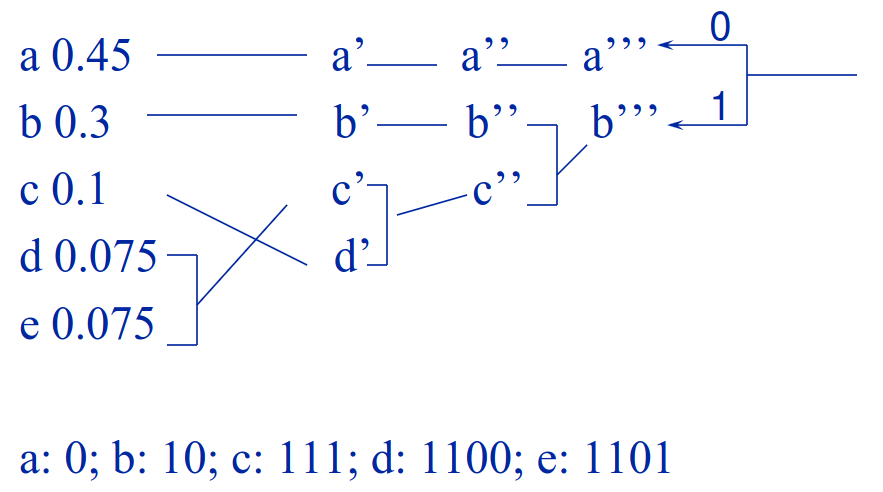
\includegraphics[width=.5\textwidth]{img/Compression/Huffman.png}
			\end{figure}
			
		\subsubsection{Lempel-Ziv}
			Utilisé dans \textit{gzip}. On regarde les données que on a déja envoyé avant et on trouve le bout déja envoyé, on va spécifier a quelle distance il se situe du point actuel sur quelle longueur il s'etend.

			\begin{figure}[H]
				\centering
				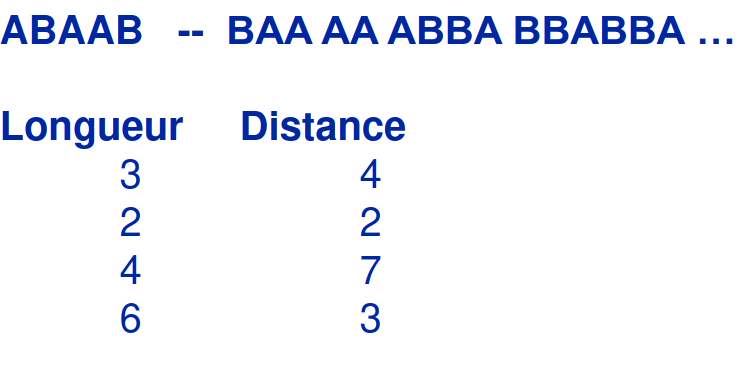
\includegraphics[width=.5\textwidth]{img/Compression/L77.png}
			\end{figure}
			
	\subsection{Codage avec pertes}
		On va mesurer une \textit{distorsion} (somme des carres des erreurs ou Distance de hamming) qui va dire le taux d'erreur acceptable. Plus il est élevé, moin on a besion de débit pour les données
		
		\subsubsection{JPEG}
			Les block de 8x8 pixel de l'image sont remplacé par des matices de coefficients DTC de taille 8x8. Le but est de perdre que une parties des blocs de DCT. Virer des pixels non mais oublier un DCT ok
			
			On applique ensuite la \textbf{quantification} sur la matrice de coefficient DCT. On divise la matrice de pixel en matrice de quantification dans le but d'atténuer les hautes fréquences (presque insensible pour l'humain). Certains coefficient sont a 0 (en bas a droite de la matrice).
			
			Ensuite un codage en ZIG-ZAG permet de ne garder qu'un minimum de coéfficient et de se débarasser des nuls.
			
			\begin{figure}[H]
				\centering
				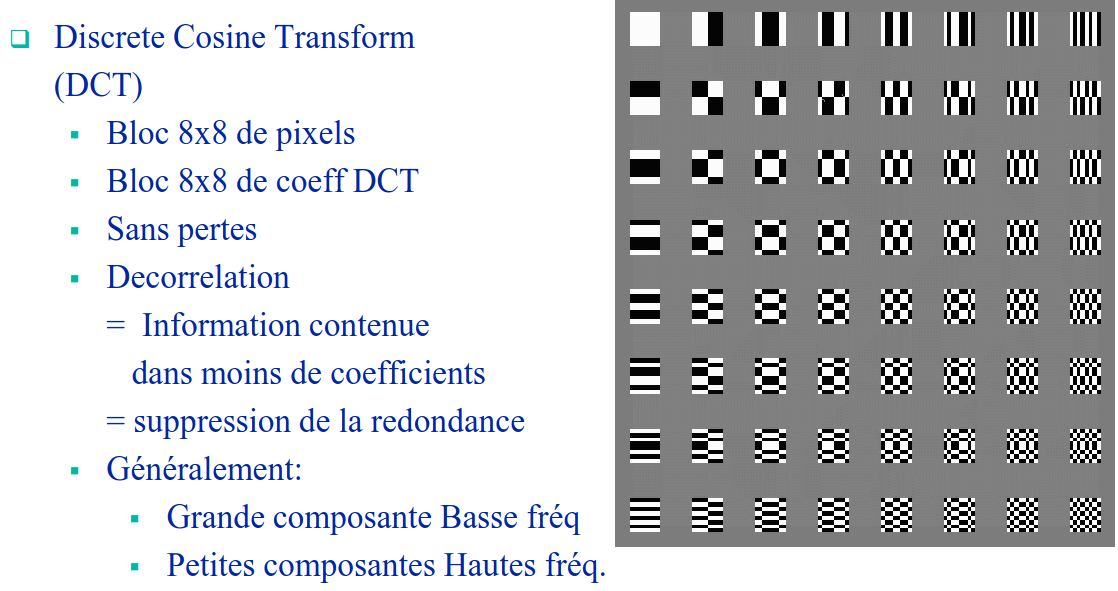
\includegraphics[width=\textwidth]{img/Compression/DCT.png}

			\end{figure}
			\begin{figure}[H]
				\centering
				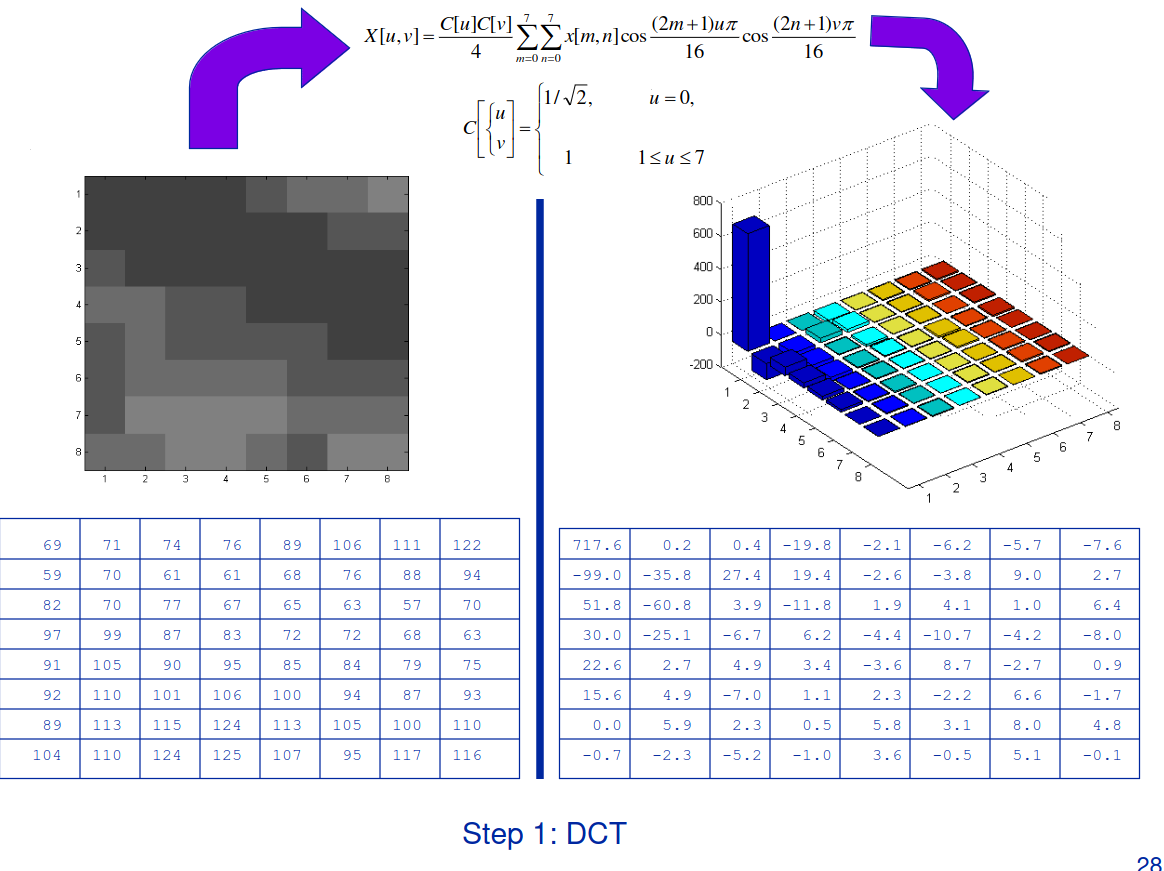
\includegraphics[width=\textwidth]{img/Compression/DCT1.png}

			\end{figure}
			\begin{figure}[H]
				\centering
				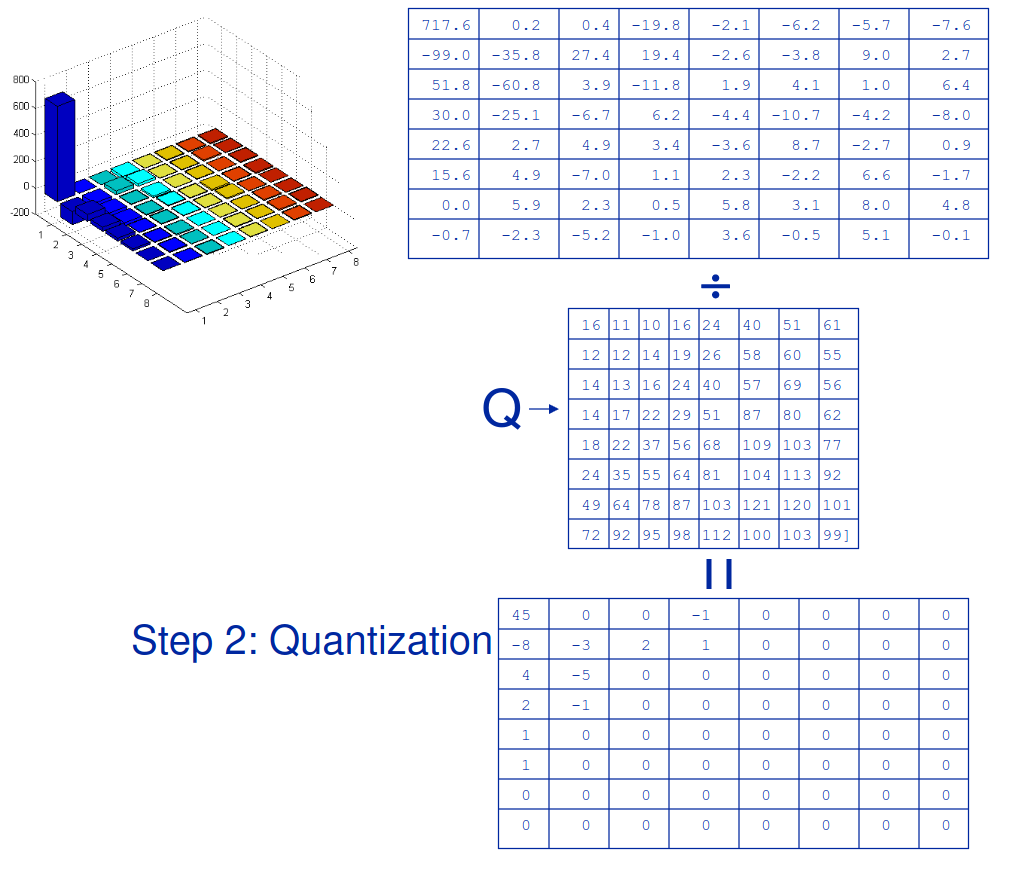
\includegraphics[width=\textwidth]{img/Compression/DCT2.png}

			\end{figure}
			\begin{figure}[H]
				\centering
				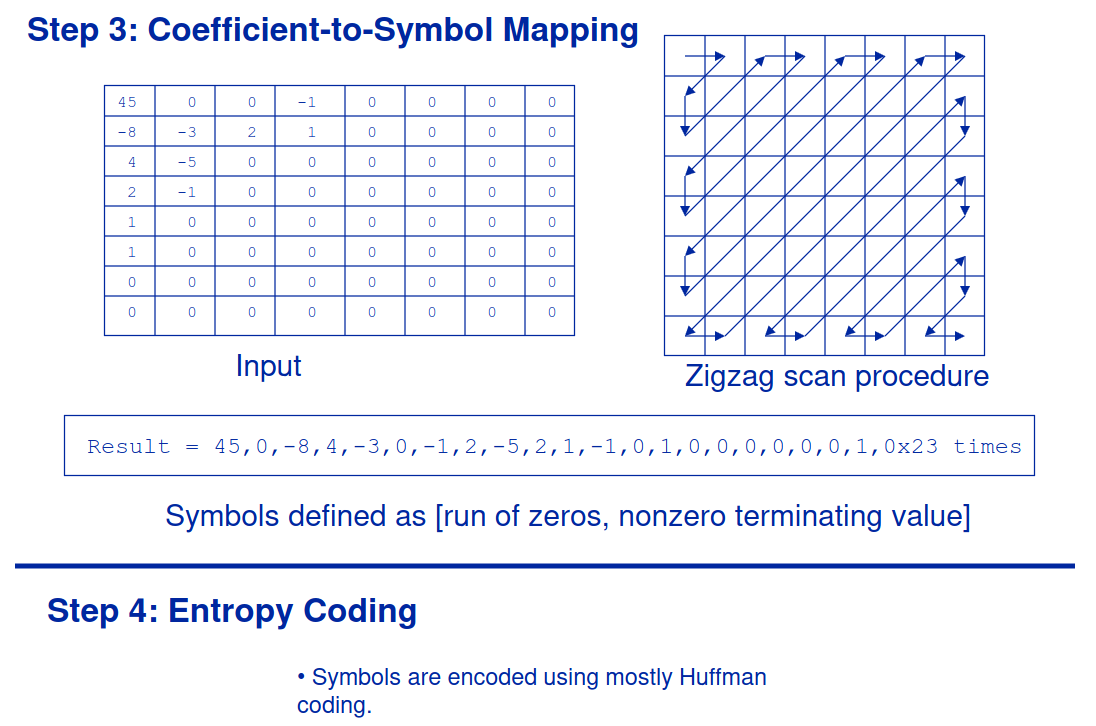
\includegraphics[width=\textwidth]{img/Compression/DCT3.png}

			\end{figure}
	\subsection{Vidéo}
		Utilise le principe de prédiction (\textbf{Block matching algorithm}). Se base sur l'idée que 2 images successive d'un vidéo sont tres peu différente. Mais pendants changement de scene, il faut garder images au complet.
		
		Un peu comme JPEG mais avec une prédictions temporelle en plus
		
		3 types de frames :
		\begin{itemize}
			\item \textbf{Intraframe (I):} Image complete (1 à 2sec) 
			\item \textbf{Interfraime (P) :} Image prédite a partir d'une précédente
			\item \textbf{Bidirect (B) :} Prédite  a partie d'un précédente ou suivante. 
		\end{itemize}
		
		La prédiction consiste en la translation d'une série de block appartenant a l'image précédente utilisé
		
		Encodage complexe et lent mais décodage tres rapide
			Fixer niveau interférence admis